
Developing retrieval-augmented generation systems is a difficult task that needs several reconfiguration phases.\cite{Simon.10112024} Component evaluation and in-depth failure analysis are key requirements for readjusting the right parts within the RAG-system, as they can include complex pipelines that may involve iterative or recursive processes. Failures can occur in many parts of the RAG-system. Barnett et al.\cite{Barnett.2024} in an advanced RAG system as Gao et al.\cite{Gao.18.12.2023} has defined it. Every additional component can increase or decrease the overall performance. Therefore for a framework it is indespensible to evaluate all components next to the end-to-end evaluation for the overall result. In this chapter, we will introduce a validate-test split for evaluation data and will justify its importance. We will discuss how RAGs are evaluated accurately in two different aspects - end-to-end evaluation and component evaluation. After that we will discuss how fast RAG development with transparent and reproducible results can be done. We will introduce Haystacks approach of fast modular RAG development via configuration files and expand its functionality for testing multiple configurations via one single file. We will present failure analysis via tracing and finally we will estimate the generalization error.

\section{Validation-Test Split}
Typical machine learning projects need the researcher to collect a lot of data, prepare it and split it into a train-validate-test split for optimizing a model with training and validation dataset and afterwards testing the generalization error done with the test dataset. The necessity of this process does not derive from training itself, but from tuning an optimizer with many free parameters to a given dataset. Whenever we try to fit data to an optimizer we need to ensure, that we did not overfit the model to a dataset. We argue that this problem is also present for RAG-systems.

No matter if training a classifier or an RAG system, both come with a large amount of free parameters. A RAG system can have hundreds to thousands of it if we include possible models for generator, embedding, corpus content or system-architectures as (indirect) free parameters. Therefore we need to ensure, that we did not overfit with our system to a given evaluation dataset. 

In this framework we will always split a given evaluation dataset via random sampling into two parts - validation and test dataset. Then we will continue to evaluate with the validation dataset and hold out the test data completely till we reconfigured to a certain satisfaction. If the reconfiguration phase is done, we will use the testset once to check if the validation error differs from the test error. The next section explains how RAGs should be evaluated to maximize its overall performance.

\section{Evaluation Techniques}

Evaluating retrieval-augmented generation systems is a hard task that is still highly researched. It comes with all machine learning based evaluation problems such as data shifts, generalization errors or data contamination, but has also a variety of failure points introduced by the design of such a complex system. In this section we will introduce a majority of failure points for RAGs and present how this framework helps to identify them. The final goal of tuning a RAG system is always to maximize its performance in end-to-end evaluation. RAG users want that the response of the systems fully answers its question or completes its task correct. 

The problem that occurs with end-to-end evaluation is that it is far from obvious which parameters we have to tune or which data we have to provide to accomplish a performance improvement. In figure \ref{fig:failures} there is an example for every component in particular RAG system. In reality there are much more points of failures in such systems. RAG systems work like real-world pipelines. We need to figure out which components are bottlenecks and swap them out with more performant ones. This can only be done with rigorous failure analysis. Therefore every experiment needs to have tracing the content for figuring out why an query was answered wrong. We are doing this with Langfuse's\cite{Langfuse} self-hosted version. We visualize all metrics and RAG parameters in MLflow\cite{MLflow}. MLflow does also contain an tracing module and an GenAI module. We decided against those features, because the tracing module is not compatible with Haystack yet and the GenAI feature requires actual ground-trugh documents which we find impractical due chunking optimization, nearly all features are marked as experimental and might be removed soon as well as our implementation of validation-test split is not compatible with this feature.

\begin{figure}
  \centering
  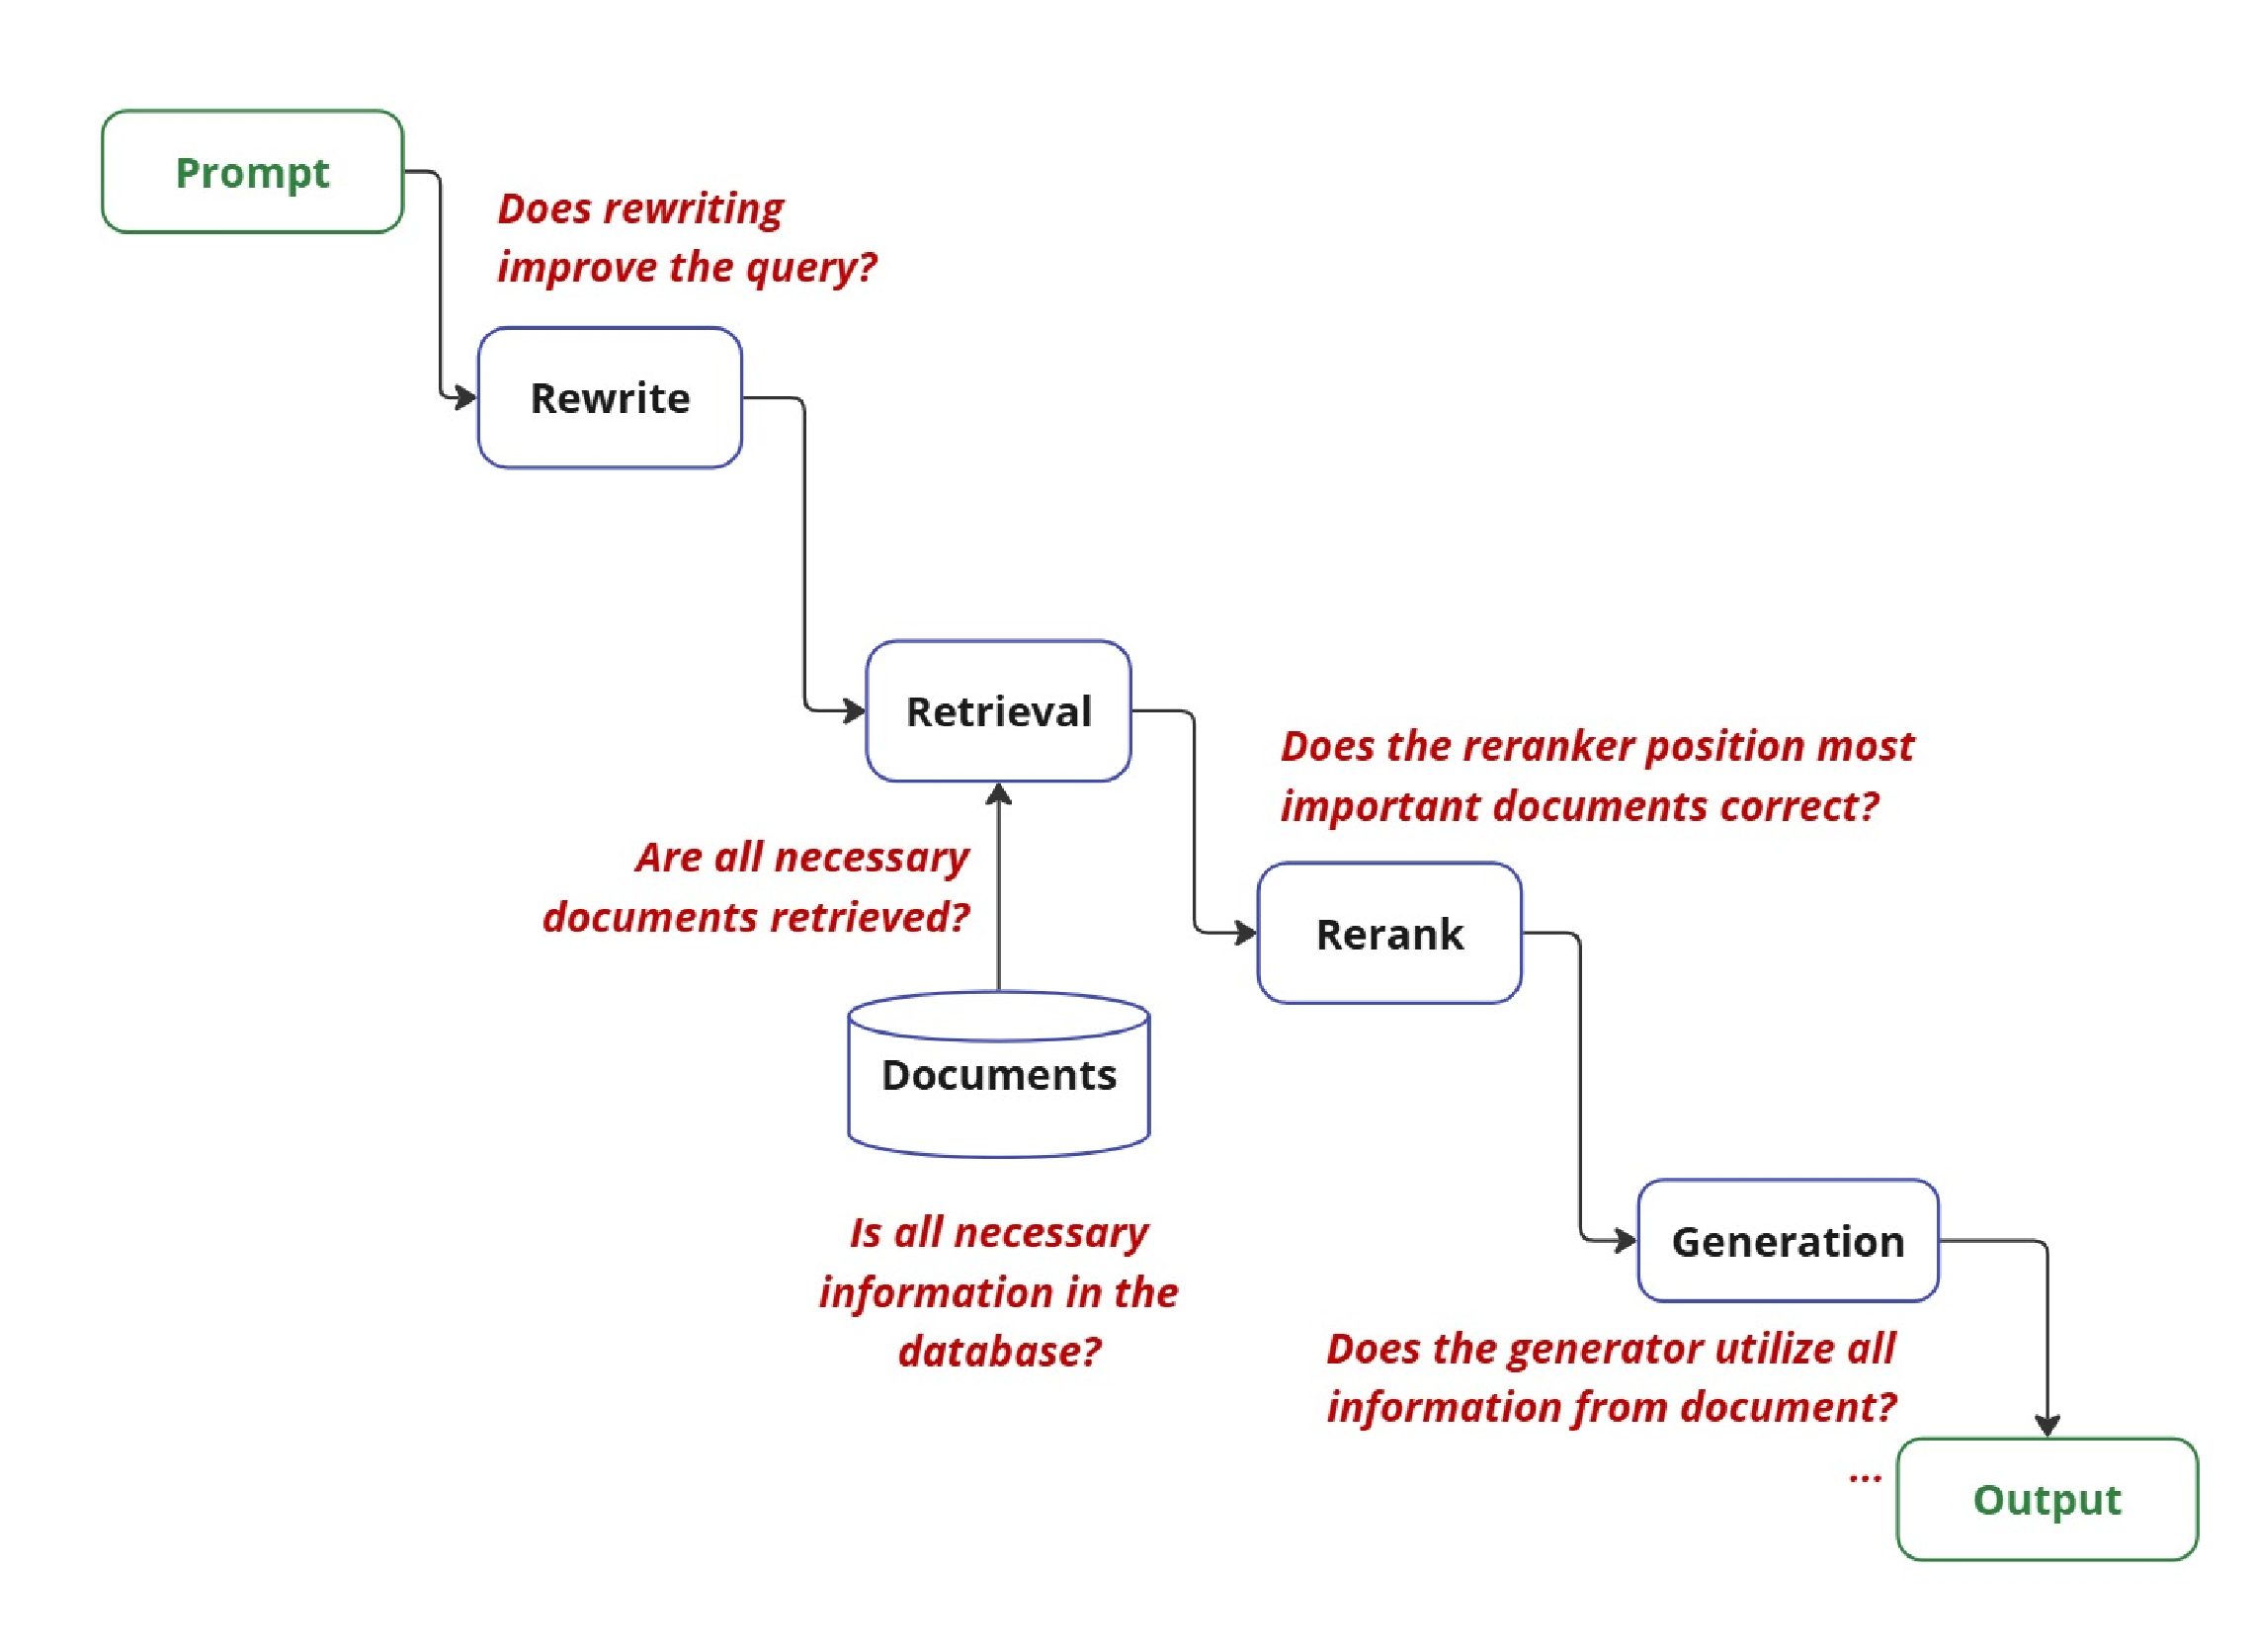
\includegraphics[width=\textwidth]{images/FailurePointExamples.pdf}
  \caption{A RAG pipeline with one failure example for each used component.}
  \label{fig:failures}
\end{figure}

\subsection{End-to-End Evaluation}

We define end-to-end evaluation as metrics that uses input and actual output to compare the result against a ground-truth output to decide if the evaluated item was correct or not. Evaluation that address retrieval or the generators ability to utilize context are therefore not part of end-to-end evaluation. In this thesis we will focus on classification tasks only. Therefore the metrics we use for end-to-end evaluations are also limited by classification ones. 

{\renewcommand{\arraystretch}{1.5}%
\begin{table}
  \centering
 \begin{tabular}{|l|l|}
  \hline
  \textbf{Metric} & \textbf{Formula / Description} \\[3pt]
  \hline Accuracy & $\frac{TP + TN}{TP + TN + FP + FN}$\\[5pt]
  \hline Precision & $\frac{TP}{TP + FP}$\\[5pt]
  \hline Recall & $\frac{TP}{TP + FN}$\\[2pt]
  \hline F1-Score & $2 \times \frac{Precision \times Recall}{Precision + Recall}$\\[2pt]
  \hline Matthews Correlation & $\frac{TP \times TN - FP \times FN}{\sqrt{(TP + FP)(TP + FN)(TN + FP)(TN + FN)}}$\\Coefficient & \\[2pt]
  \hline False-Positive Rate & $\frac{FP}{FP + TN}$\\[2pt]
  \hline False-Negative Rate & $\frac{FN}{FN + TP}$\\[2pt]
  \hline Receiver Operating & \textcolor{red}{Curve plotting TPR against FPR at various} \\&threshold settings\\[2pt]
  \hline Area under ROC Curve &  \textcolor{red}{AUC of the ROC curve}\\[2pt]
  \hline
 \end{tabular}
 \caption{Typical classification metrics used for experiments including RAGs or LLMs\cite{Hou.8212023,Zeng.28.03.2024}}
 \label{table:classification_metrics}
\end{table}}

In stark contrast to evaluating generative tasks, classification comes with clear metrics or methods to evaluate outputs. In table \ref{table:classification_metrics} there is a list of highly used classification metrics for RAG and LLM experimentation.\cite{Hou.8212023,Zeng.28.03.2024} 

End-to-end evaluation requires the researcher to establish a \textit{baseline} for the experiments. Baslines make experiment results interpretable and ensure that there is something to compare with. Therefore we decided to implement two baselines in this framework, which are used per default if an experiment starts. The first baseline consists only of a standalone LLM. The second baseline is a naive RAG with BM25 retrieval and with the data from the predefined corpus (retrieve-read, cf: section \ref{sec:naive_rags}). The standalone LLM baseline ensure that the complexity overhead of implementing a RAG system is justified. If the evaluated RAG system can not surpass the performance of the LLM baseline, then simpler system should be used. Advanced RAGs often need more components, which result in longer computing times and costs. Outperforming the naive RAG ensures that simple but fast retrieval alone is not sufficient. 

\begin{figure}[h]
  \centering
  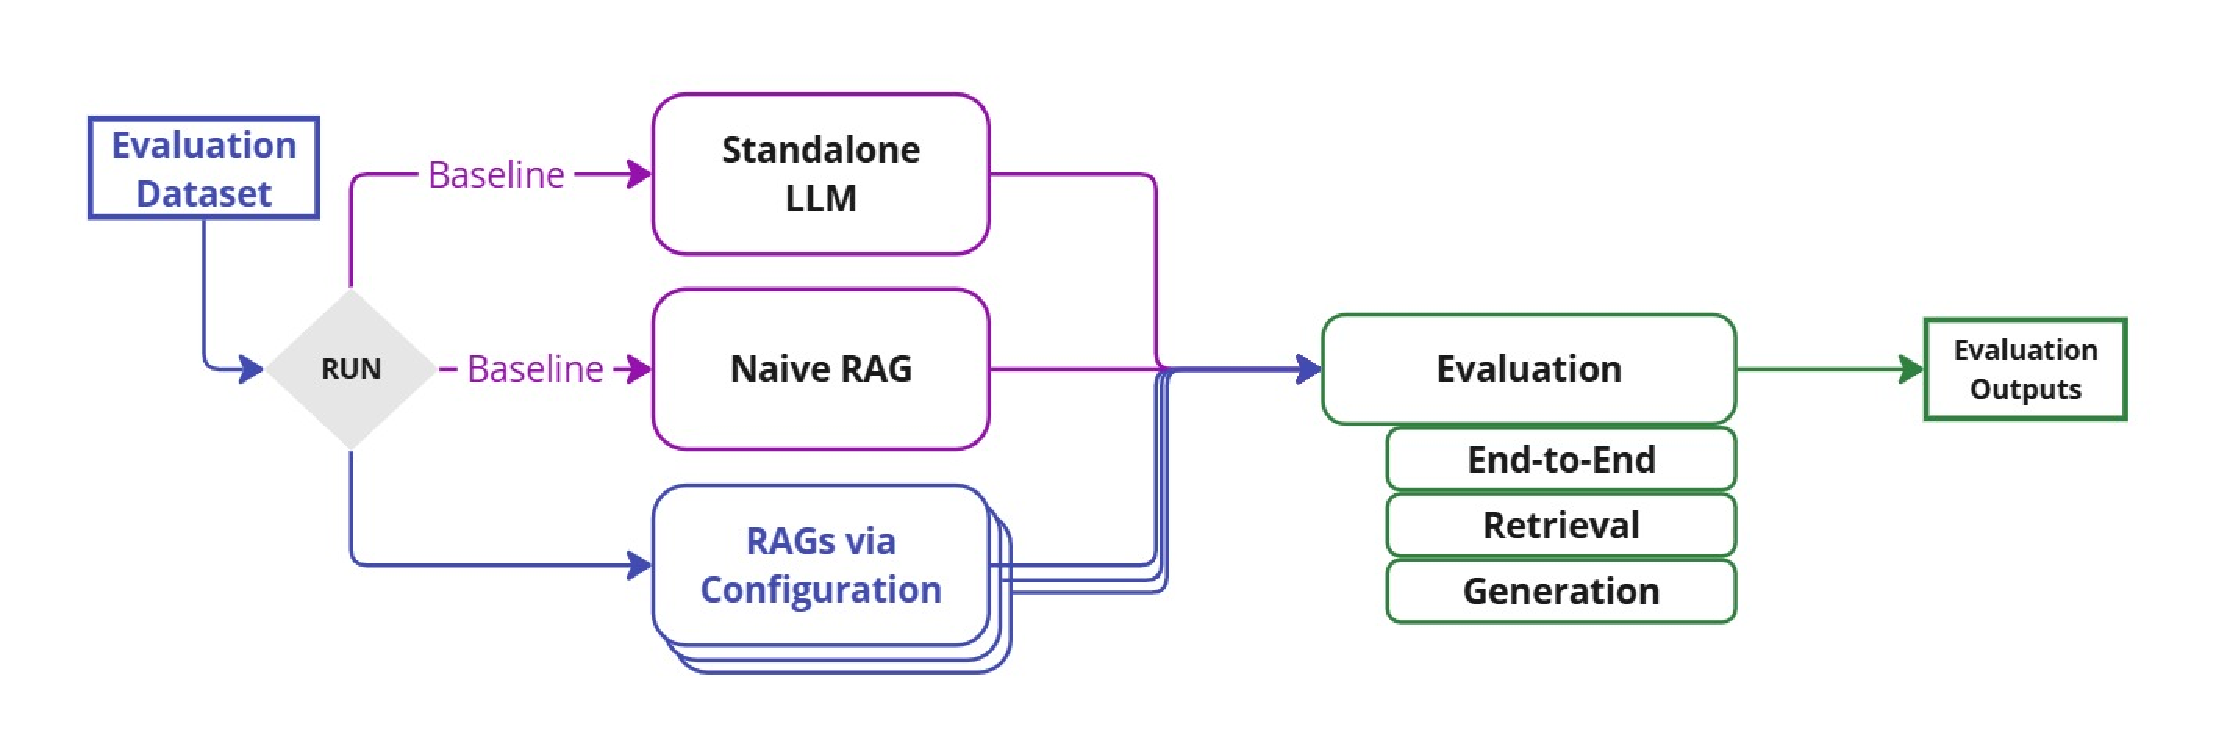
\includegraphics[width=\textwidth]{images/FrameworkBaselines.pdf}
  \caption{Framework: research define configuration files of RAG variations to evaluate them against the baselines standalone LLM and naive RAG with end-to-end evaluation.}
  \label{fig:framework-baselines}
\end{figure}
% \cite{Ru.15.08.2024.} Eventhough all components of a RAG-system affect its overall performance, there are ones that can not be evaluated directly.  \\

We illustrated the prior defined state of our framework in figure \ref{fig:framework-baselines} to enhance the understanding of our considerations. It will be updated with each functionality. It visualizes the process of using our evaluation data to calculate metrics of our baselines next to the configurations we want to test in the experiment. It shows that the evaluation is done by end-to-end as well as component-wise for generation and retrieval. In the following section we will explain, how component evaluation works in our framework.


\subsection{Component Evaluation}

Component evaluation is necessary to detect performance issues of the whole systems introduced through individual components or blocks of components that are connected and do not work well together.\cite{Salemi.2024} In figure \ref{fig:failures}, we presented few of them. While this gives a good first impression of the variety of failures in a RAG system, this visualisation is far from complete. We argue that all components, no matter how small their impact seem, can introduce significant failure rate for the overall system. Therefore it would be necessary to evaluate them all component-wise. 

We are not aware of papers that analyze component evaluation beside retrieval and read - the core components of a RAG system. We also want to make clear, that evaluating components fully isolated by other components is not practical. If we take for example the generator component and want to evaluate it completely apart from retrieval, then we must provide a ground-truth dataset of retrieval chunks. This is doable for easy scenarios in retrieval that need one document chunk e. g. a sentence where a query is exactly answered, but in real-world scenarios there are much more complex cases such as ambigious queries, complex queries or queries that won't need retrieval at all.\cite{Huang.2023} If the researcher adjusts chunk size or technique, then he must also create a new set of ground-truths as the generated documents have changed and the previous selected ones do not exist anymore (cf. section \ref{sec:advanced_rags}). 

If we consider other components then retriever such as rewrite or rerank then there is no ground truth of data. The purpose of rewriting the query is increasing the following retrieval. Therefore the metric is dependend on the retrieval technique too can not be fixed ground truth examples in an evaluation dataset.

The purpose of component evaluation is to find weak spots within the RAG. It is therefore more feasible to evaluate a RAG-system only with system inputs and its ground truth final answers and let a non-deterministic LLM-as-a-Judge evaluate for steps within the RAG-system. LLM-as-a-Judge is a evaluation techniques, where a significantly more performant model or solely on evaluating trained model does the evaluation. Instead of real-valued metrics, an LLM decides and asseses the solution of the task. 

Relying only on system input and ground-truth datasets for evaluation saves a lot of time. Resulting failure analysis of the system and its components must nevertheless rely on tracing single pipeline runs down, which we will discuss in a latter section. In the following sections we will present our evaluation of the retrieval block and the generation block.


\paragraph{Retrieve}
Retrieval Evaluation is possibly the most difficult part in the evaluation for several reasons. First, more retrieval do not imply better results and it is not clear nor obvious which set of documents perfectly serves the generator to give the best answer.\cite{Jin.5222024} Second, in a real world scenario indexed corpus, there are redundant and contradicting information.\cite{Yu.2024} Third, some questions or queries require to view the topic in a diverse manner, highlighting several considerations for different perspectives and fourth, the quality of the query does also affect the retrieval quality, because queries can be too complex and ambigious or not even requiring retrieval, which may also lead to LLM hallucinations.\cite{Huang.2023, Mallen.20.12.2022}

Retrieved documents might contain useful information or not and are therefore binary assessable, enabling metrics that handle \textit{True-Positives, True-Negatives, False-Positives} and \textit{False-Negatives}. However, simple metrics such as recall and precision are not suited to measure the small differences in retrieval.\cite{Yu.2024} There is a need for retrieval evaluation techniques that also capture document rank information.

Additionally there are limitations while working with ground-truths in retrieval evaluation. Ground truth context for a given query might be ambiguously. Selecting a ground-truth set of relevant information is a task that even expert humans are not able to solve perfectly and LLM-as-a-Judge models show high correlation with humans.\cite{Chiang.2023} There is also the problem of changing chunking while reconfiguration. Everytime a chunking technique or parameter is changed, the resulting indexed documents are different too. Therefore it would be required to prepare a new evaluation dataset for ground truth retrievals. This is a great bottleneck for fast reconfiguration cycles, but chunking is a very important parameter to tune. Therefore we will focus in this framework solely on LLM-as-a-Judge evaluation for retrieval to enable chunking parameter tuning.

We utilize a metric called \textit{Context Relevance} (sometimes also referred to as \textit{Context Precision} or similar names in different frameworks), which is fundamentally a Mean Average Precision (MAP) metric employing an LLM-as-a-Judge. This metric assesses the relevance of each retrieved document in relation to a given query. A binary approach is often adopted, where the LLM-as-a-Judge determines for each document whether it is relevant or not. Specifically, frameworks like Haystack's `ContextRelevanceEvaluator`\cite{Pietsch_Haystack_the_end-to-end_2019} implement this binary assessment. For each document, the evaluator determines if it contains any statements relevant to the query. If relevant statements are found, the document is considered relevant (score 1), otherwise not relevant (score 0). The final \textit{Context Relevance} score is then calculated as the mean of these binary relevance scores across all queries, effectively representing a form of Mean Average Precision. While some frameworks like RAGAS might calculate retrieval metrics based on the quality of the generated response, the approach used here and in Haystack focuses directly on evaluating the relevance of the retrieved documents themselves using a binary LLM-as-a-Judge assessment.

We stated before that recall can not fully capture a complex task like retrieval. Therefore we implemented also \textit{Mean Average Precision at K documents MAP@K}, a custom \textit{Context Precision} metric to offer a complementary, rank-agnostic perspective by simply measuring the proportion of relevant documents retrieved. This additional metric ensures a more comprehensive evaluation of retrieval performance, capturing aspects beyond ranking quality.\cite{EvidentlyAIInc..25.02.2025} 

$$MAP@K=\frac{1}{|Q|}\sum_{q=1}^{|Q|}AP@K$$
$$AP@K=\frac{1}{N}\sum_{k=1}^{K}Precision(k) \cdot rel(k)$$
\begin{itemize}
  \item $|Q|$ is the total number of queries in the evaluation set.
  \item $q$ represents a specific query from the set of queries.
  \item $AP@K$ is the Average Precision at K for a specific query.
  \item $N$ is the total number of relevant items for a particular query.
  \item $K$ is the number of top documents being evaluated.
  \item $k$ represents a specific position in the ranked list of retrieved documents.
  \item $Precision(k)$ is the precision calculated at position $k$, defined as the number of relevant items among the top $k$ items divided by $k$.
  \item $rel(k)$ equals 1 if the item at position $k$ is relevant and 0 otherwise.
\end{itemize}

This is a modified version of the \textit{MAP@K}.\cite{Lin.13.10.2020} It is usual to set K very high and let it retrieve a lot of documents to ensure the relevant ones are retrieved. This would be in conflict with the prior defined \textit{Context Precision} metric. Therefore we will only calculating \textit{MAP@K} for the real k value. \textit{Context Precision} measures the retrieval quality based on focussing to retrieve only relevant items and \textit{MAP@K} measures the ranking inside the retrieved documents. A low \textit{Context Precision} and a high \textit{MAP@K} indicate that the paramter \textit{Top-K} can be reduced, because the retrieval works well enough that irrelevant documents appear on the bottom of the retrieval. In contrast a low \textit{MAP@K} could suggest, that the retrieval configurations is not well-adjusted enough, because there are too many irrelevant documents on the top of the retrieved list.

\begin{figure}
  \centering
  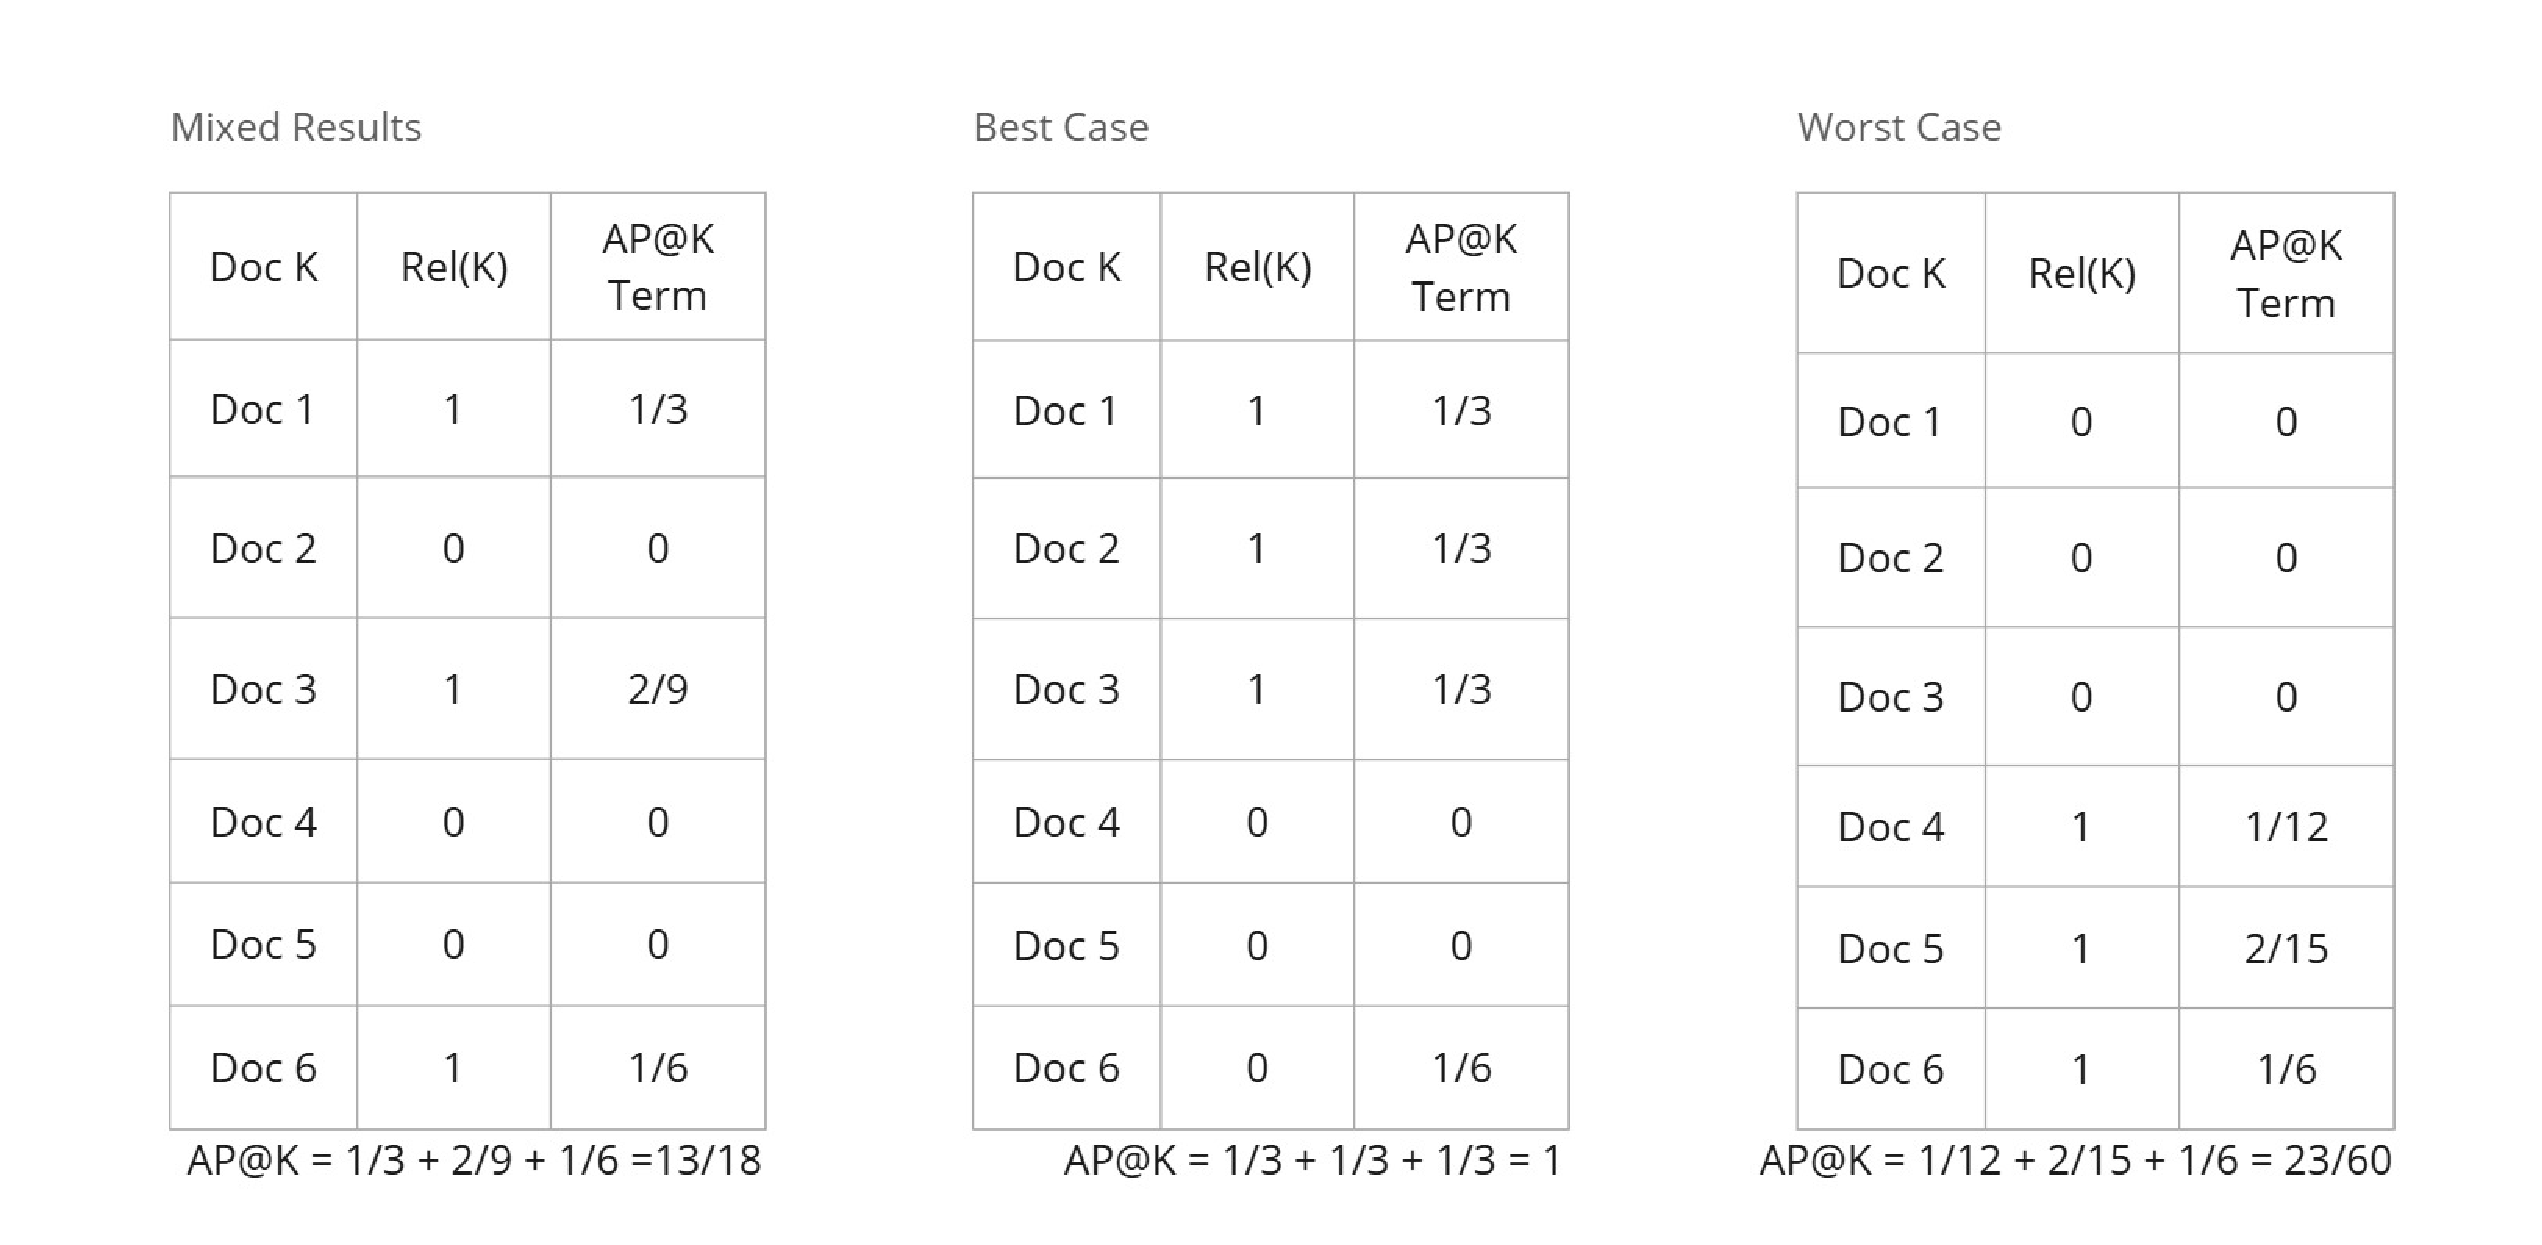
\includegraphics[width=\textwidth]{images/APatK.pdf}
  \caption{This is an example for AP@K metric for one query. At each retrieved document relevance and precision of the first to K-th document will be averaged through all retrieved documents.}
  \label{fig:APatK}
\end{figure}


\paragraph{Generators}
Generators are based on transformer architecture and classification tasks were not the initial intention for this kind of tasks. Thus it is important that outputs are in a wanted form such as \textit{valid}, or \textit{invalid}. Therefore we need a metric that evaluates the generators ability to follow those rules. We call this \textit{format-validator}. The problem that comes with this generator evaluation for classification tasks is that it is impossible to check context utilization, answer relevance based on a simple \textit{True/False} answer. 

Even though the generator only predicts \textit{True/False}, the latent space that lead to this answer have different grades of context utilization and answer relevance. Therefore we will use a slightly different format for the classification task. Instead of generating only binary outputs such as \textit{0} / \textit{1}, \textit{valid} / \textit{invalid} or \textit{True} / \textit{False}, we will also output the reason for it before or afterwards. The only limitation is that the model must generate \textit{'The answer is "True"'}. We implement it with an regular expression.

This has several positive side affects. First, we can measure the reasoning to assess context utilization or answer relevancy, which are important to debug the system. If the context of retrieval is not utilized enough, then we won't figure that out by analyzing binary classes. Second, we enable reasearchers to the current test-time compute paradigm shift for large language models or \textit{large reasoning models}. In practice, they use \textit{<think>...</think>} and use different search algorithms for the best reasoning path before these model answer the query. This leads to significantly better results.\cite{Xu.16.01.2025}


\subsection{Component Block Evaluation}

After evaluating component-wise, we need to evaluate other components, that are not assessable isolated too. In an advanced RAG such a component would be the rewriter. Rewriters try to synergize query to retrieval and context. Defining a performant rewriter depends on whether the RAG uses a sparse or a dense retrieval as he must either use relevant keywords or simulate semantic similarity. The second component from an advanced RAG system would be reranking. Both, reranker and generator have an great impact and interest in context utilization, the ability to build a coherent and correct answer based on actual facts from the retrieved context. Phenomena such as lost-in-the-middle have a significant affect on context utilization, but LLMs differ in this effect.\cite{Liu.06.07.2023} Therefore it might happen that the best reranker and generator regarding their component-wise performance lead to inferior context utilization results. The system needs to be model-agnostic for all components and researchers need rigorous testing of potential component blocks. 

\paragraph{How to evaluate such component blocks?}

\begin{figure}
  \centering
  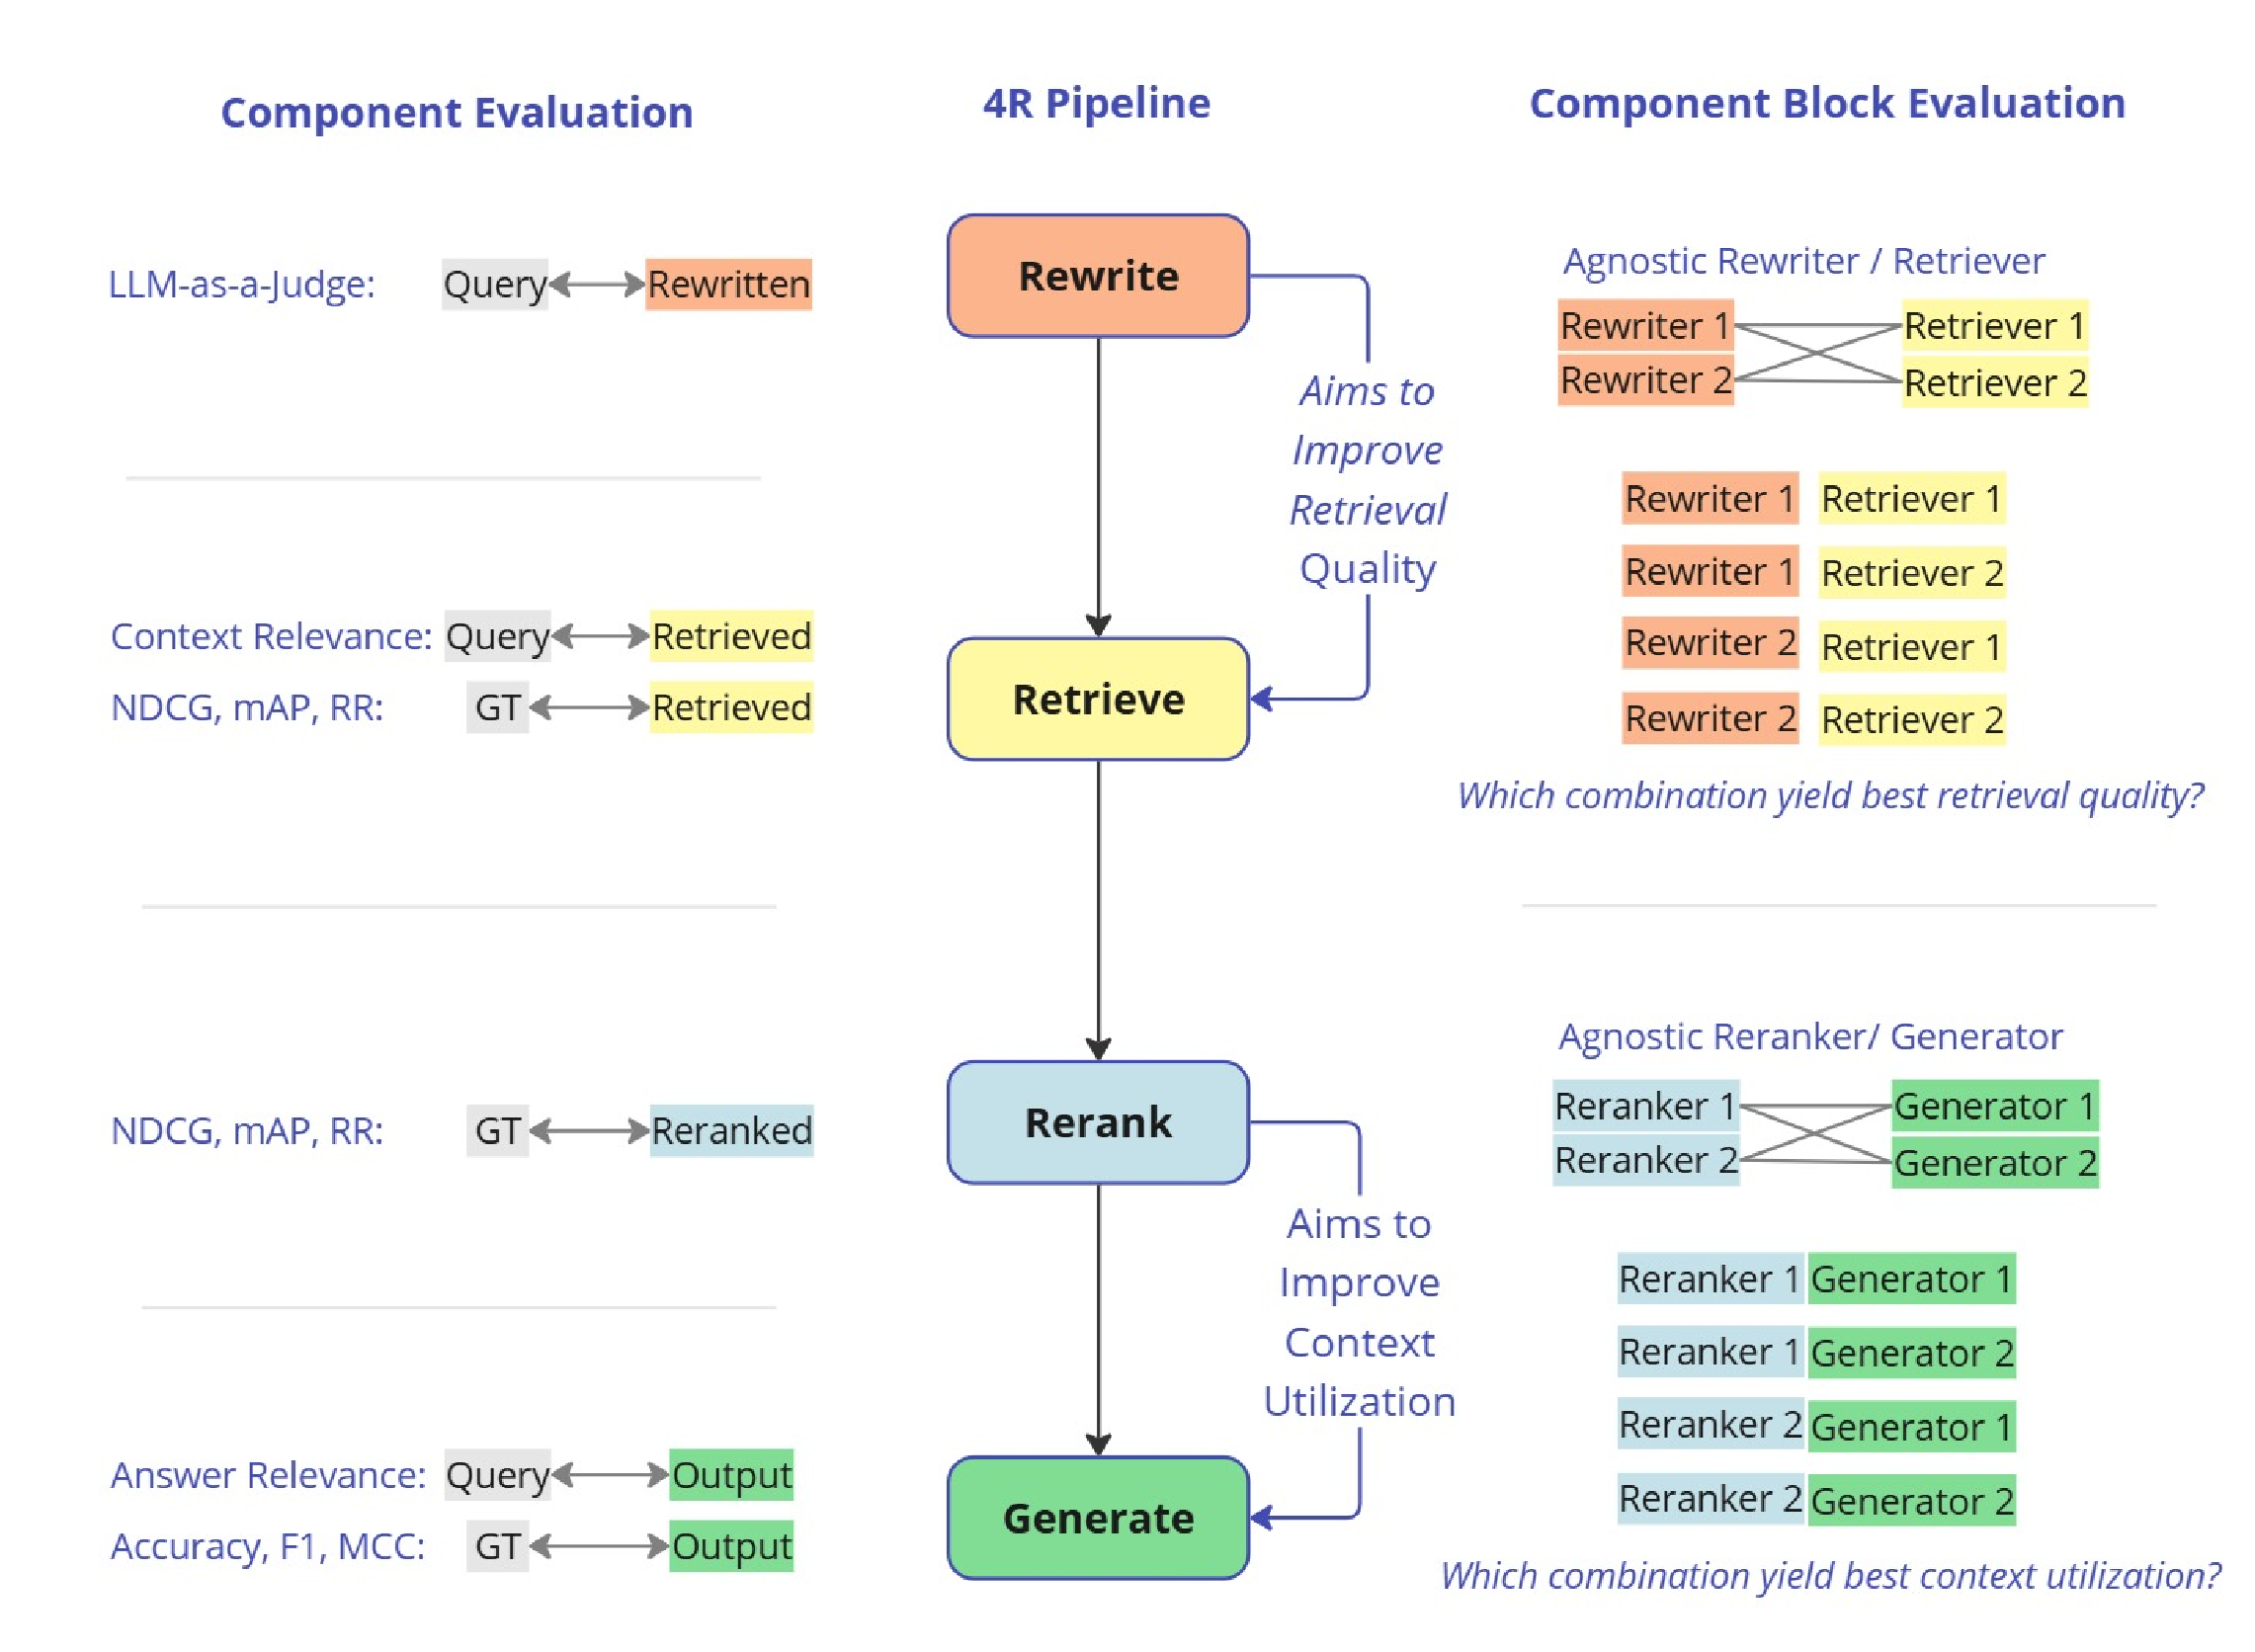
\includegraphics[width=\textwidth]{images/ComponentBlockEvaluation.pdf}
  \caption{Comparison of isolated component evaluation of each component and component block evaluation, where several components with the same goal are evaluated.}
  \label{fig:componentblockeval}
\end{figure}


We differentiate two major blocks - pre-retrieval and post-retrieval. Evaluating pre-retrieval component blocks such as rewriter is a derived task from the retrieval evaluation. The goal of pre-retrieval is to increase the retrieval quality so that the retriever finds all necessary documents or chunks for this task. Commonly used pre-retrieval techniques are query routing, query transformation and query expansion. Even in the ingestion stage, chunking, document selection and preprocessing steps are tuning parameters that influence retrieval results and its quality. 

Post-retrieval components such as reranker aim to improve the context utilization for the generator. The generator requires a curated and limited list of documents that serves its ability and query best. Second, reducing the Top-K parameter for retrievers might result in missing documents with required information. For that we use the same metrics as for the retriever. The additional step of reranking influences the overall performance and evaluating this component is important. 

Most components beside retriever and generator have no direct measurement,there they have to be evaluated by replacement and metrics of the component block. For example, the rewriter is evaluated by using similar components, different models or prompting techniques as rewriter-variations. Then the RAG runs through the evaluation by only changing those rewriter specific configurations. The resulting end-to-end or if applicable the resulting retrieval metrics decide which rewriter setting is better suited. This approach requires the researcher to try many different RAG variations for rigorous testing. In the next section we will introduce our appraoch for fast RAG development.

\section{Fast RAG Development}

\begin{figure}[b]
    \centering
    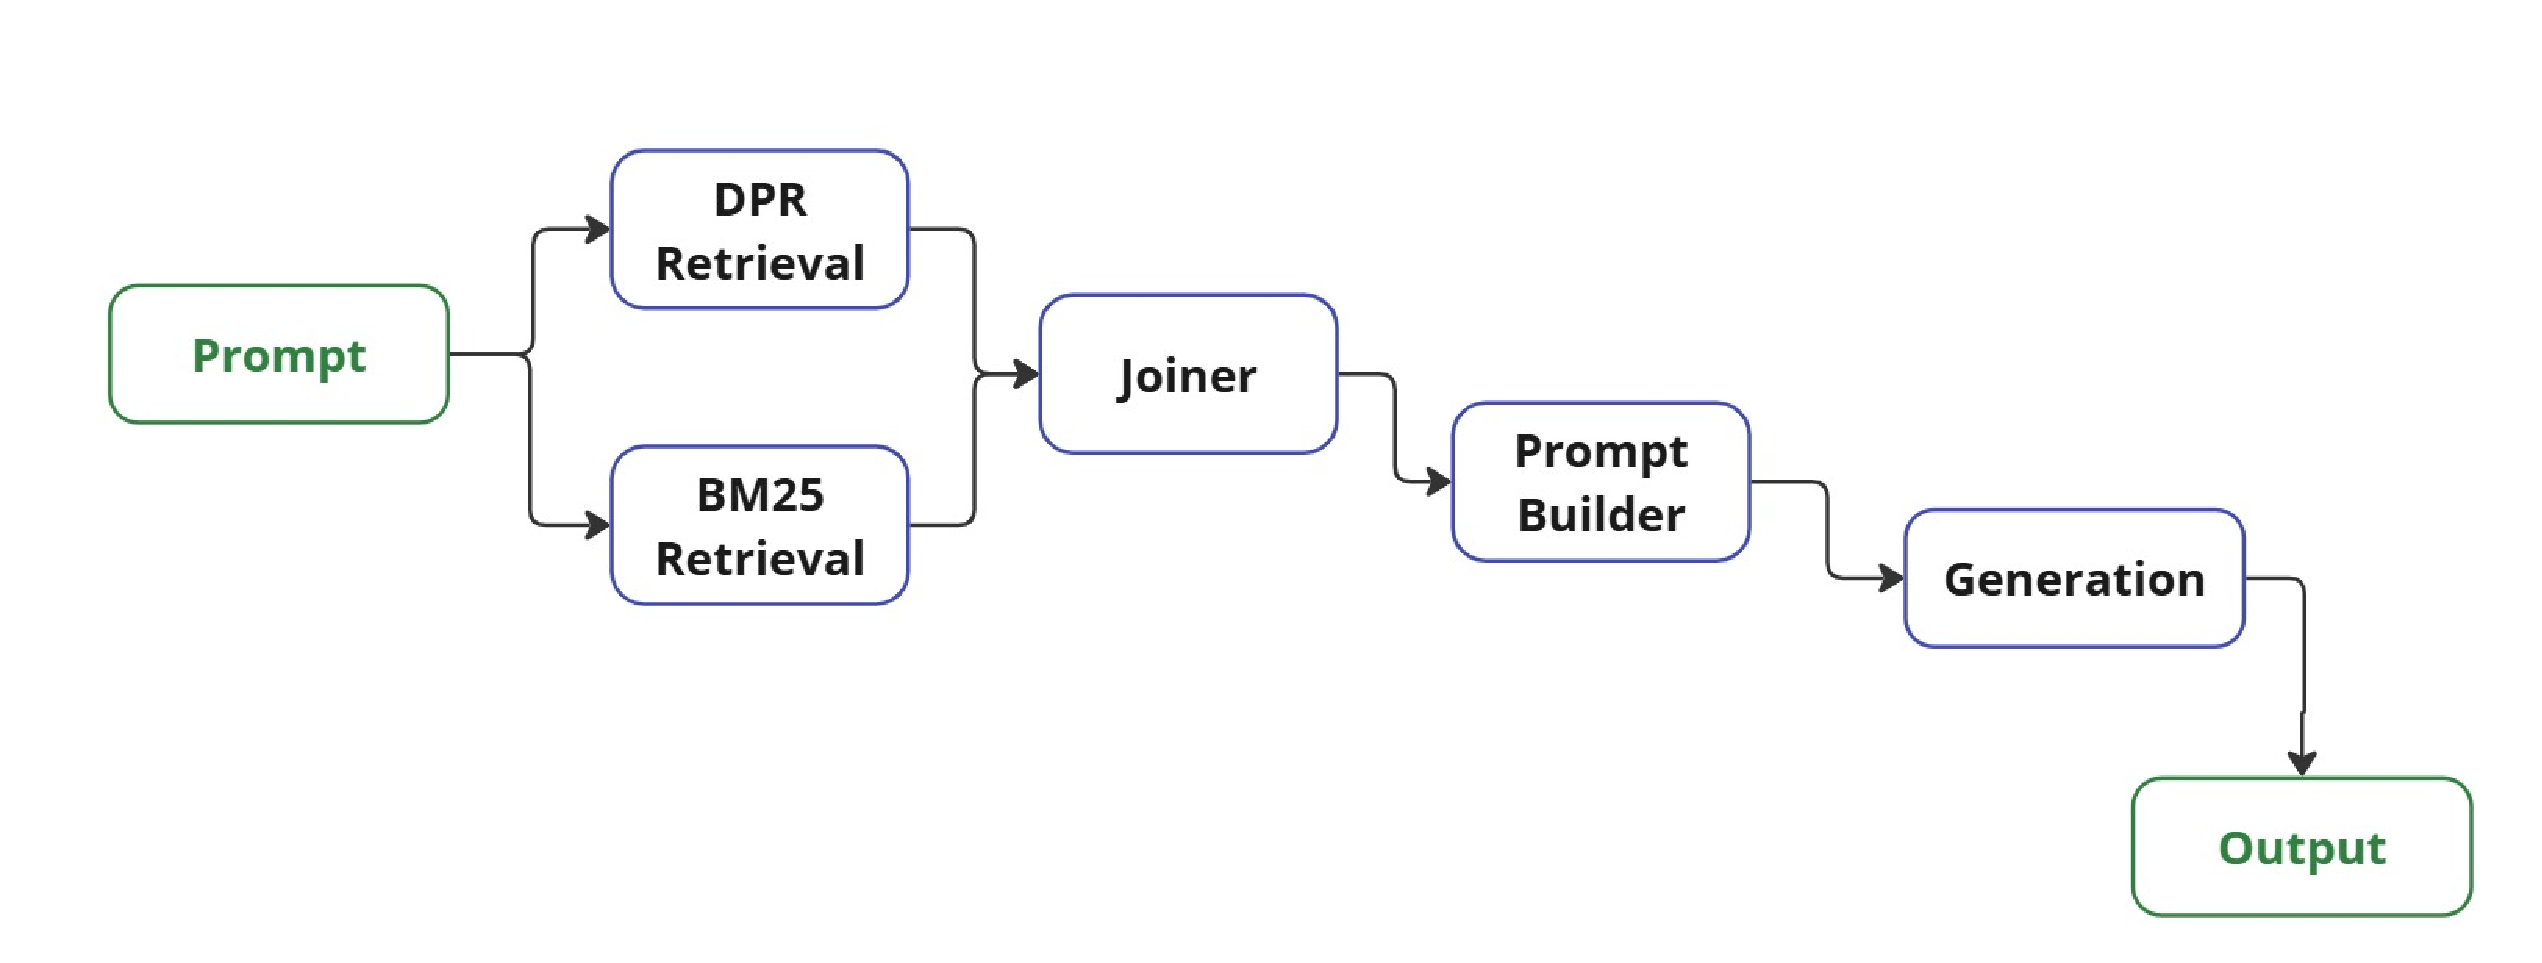
\includegraphics[width=\textwidth]{images/showcase-pipeline.pdf}
    \caption{A simple Retrieve-Read pipeline with both dense and sparse retrieval.}
    \label{fig:showcase}
\end{figure}

RAG systems have a lot of parameters that are not obvious to set. It is common as a researcher to have several reconfiguration phases till the RAG systems works sufficient. More reconfiguration phases lead logically to better results. Therefore Short feedback cycles and fast development make it possible to evaluate many configurations and short feedback cycles can lead to fast bottleneck improvements. This sections presents our considerations for offering fast RAG development.

There are several RAG development tools and frameworks. Highly used ones are Llama-Index\cite{Liu_LlamaIndex_2022}, Langchain\cite{Chase_LangChain_2022} and Haystack\cite{Pietsch_Haystack_the_end-to-end_2019}. All of them offer comparable functionality for building advanced RAG systems in modularized architecture as introduced by Gao et al.\cite{Gao.18.12.2023}. Haystack comes with custom components that enable new component technologies and does offer a functionality, where users can define a pipeline via a YAML-file. This enhances the reconfiguration of such systems, because instead of editing python files, there are just parameters in one YAML-file to be changed. This enhances the ability to report the methodologies of each experiment too. Instead of saving a python script or module for each configuration, only a YAML is stored that describes the tested RAG architecture fully. An example of this YAML definition can be seen in figure \ref{fig:showcase} and the YAML code below.

There are are more benefits for configuring via YAML files. First, we can copy existing RAG configurations easily. Second pipeline definitions can still be done in python, saving the afterwards into the YAML format. Lastly, Haystack develops an UI\cite{haystack-ui} for developing RAG system, that can be used to create such complex systems on a two-dimensional space.

\begin{minted}[
    frame=single,
    bgcolor=lightgray
  ]{yaml}
components:
  llm:
    init_parameters:
      api_base_url: null
      api_key:
        env_vars: OPENAI_API_KEY
      ...
  prompt_builder: ...
  bm25_retriever: ...
  embedding_retriever: ...
  joiner: ...
  text_embedder: ...
  docs_embedder: ...
  answer_builder: ...
connections:
- receiver: llm.prompt
  sender: prompt_builder.prompt
- ...
\end{minted}

While copying configuration files and adjusting parameters of it is more efficient then handling verbose python modules, we expanded haystacks core functionality for saving and loading YAML configurations with matrix notation.
We allow different parameters within a list and generate all possible combinations of that configuration. In the example below we can see 4 different combinations: ("gpt-4o-mini", 5), ("o3-mini", 5), ("gpt-4o-mini", 10) and ("o3-mini", 10). This ensures that the researcher can try and validate many different models or parameters and compare their impact on the overall performance.

\begin{minted}[
  frame=single,
  bgcolor=lightgray
]{yaml}
components:
  llm:
    init_parameters:
      model: ["gpt-4o-mini", "o3-mini"]
      ...
  retriever:
    init_parameters:
      top-k: [5, 10]
  ...
\end{minted}

% The visualisation shows the process of reconfiguring the RAG system till its optimized towards a specific validation set. The reconfiguration phase can adjust parameters, using different models, pipelines or even fine-tuning parts such as retriever or generator. We will introduce detailed validity concerns of this common approach in a latter section. 

\begin{figure}[h]
  \centering
  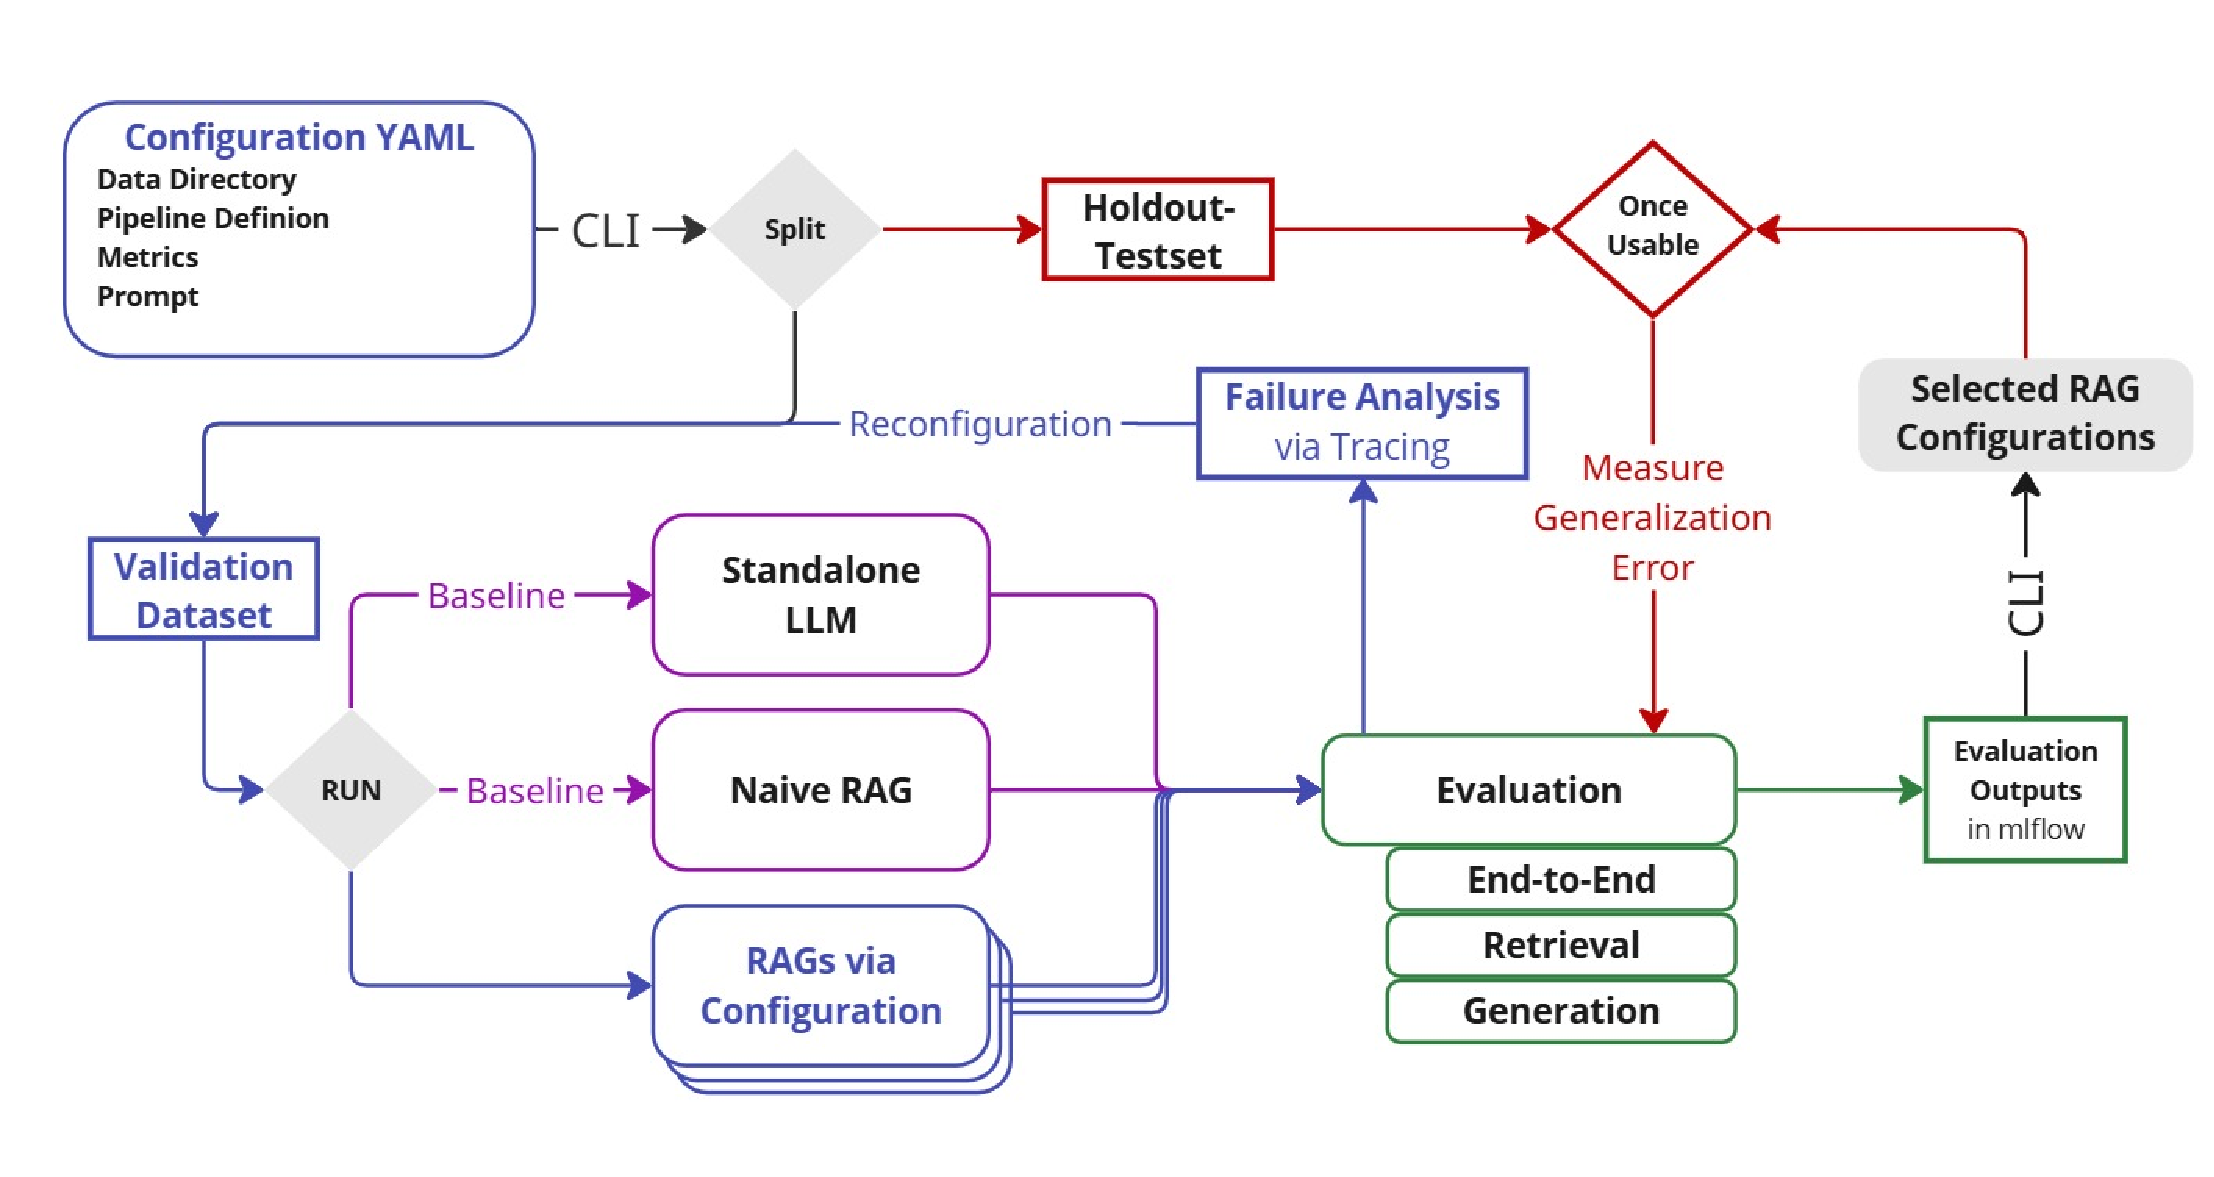
\includegraphics[width=\textwidth]{images/FrameworkFull.pdf}
  \caption{Framework: At first the evaluation data get splitted into validation and hold-out test dataset. Then the validation data is used to evaluate a configured RAG system and compare it against baselines. After failure analyisis several reconfiguration phases can happen. At last the test dataset is used to test all configurations for a potential generalization error.}
  \label{fig:framework-full}
\end{figure}


\section{Transparency}

We are following Simon et al.\cite{Simon.10112024} recommendations for ensuring transparency in RAG experiments. First we ensure that the used data is either publicly availlable or published by the experimenter. This does not fall under the functionality of this framework, because this is usually done via version control such as Github\cite{github-inc-2025} or Gitlab\cite{gitlab-inc-2025}. Another popular decision is DVC\cite{dvc.17.03.2025}, which is primarly focussed on machine learning experiments and therefore less suited for RAG development. Their approach of adding stages is a lot of overhead that might be too time-consuming for fast RAG development. Beside that derived features such as visualisation are adjusted to training which is epoch-oriented. 

Code as well as RAG-system architecture is saved with each commit. This ensures that every configuration phase can be restored as well as transparently reported. 

We added in all configuration files meta data parameters. We highly recommend this practice for every configuration phase. There can be written down comments, hypothesis or simple thoughts that can later on be used to compare different results within MLflow. Additional this can be used to make it more transparent why this reconfiguration phases were executed. This has several benefits.
At first, it makes researchers intentions more clear e. g. did the researcher wanted to improve retrieval or context utilization? 
Second, it also shows unsuccessful configurations or hypothesis, which can be used by other research teams later on.

Typical machine learning experiments require seeding, which can be complicated as it is not clear which services support it. We included it in the openai generators in our example configurations and want to raise attention for including seeding in all applicable situations.

The here stated transparency considerations and actions make sure that RAG experiments are reproducible as much as we can. It assumes a static dataset. If the dataset is frequently changing the users needs to use a workaround with DVC, which we have decided not to include.
Beside that all experiments are reproducible as long as all components of the system that include randomness can pass a seed parameter.

\section{Validity}

\paragraph{Internal Validity}
Evaluating semantics in LLM's or RAG systems rely on LLM-as-a-Judge models or lexical metrics such as BLEU or ROUGE, which measure the token overlap of actual answer and ground truth. Lexical answers can not capture answer pairs that are differently written but having the same semantic. LLM-as-a-Judge are on par with human-level judging, but are prone to preference leakage. There are findings suggesting that LLM-as-a-judge favor similar LLMs that their based on. Therefore using synthetic data for evaluation is fast, but risks preference leakage.\cite{Li.03.02.2025} This field is very new and still under research. We implemented our LLM-as-a-Judge metric for context utilization with environment variables that default to OpenAIs \textit{gpt-4o-mini}\cite{OpenAI_2022}. We warn users actively about this potential bias and let them have the possibility to vary the generator model family from the LLM-as-a-judge model family.

\begin{figure}
    \centering
    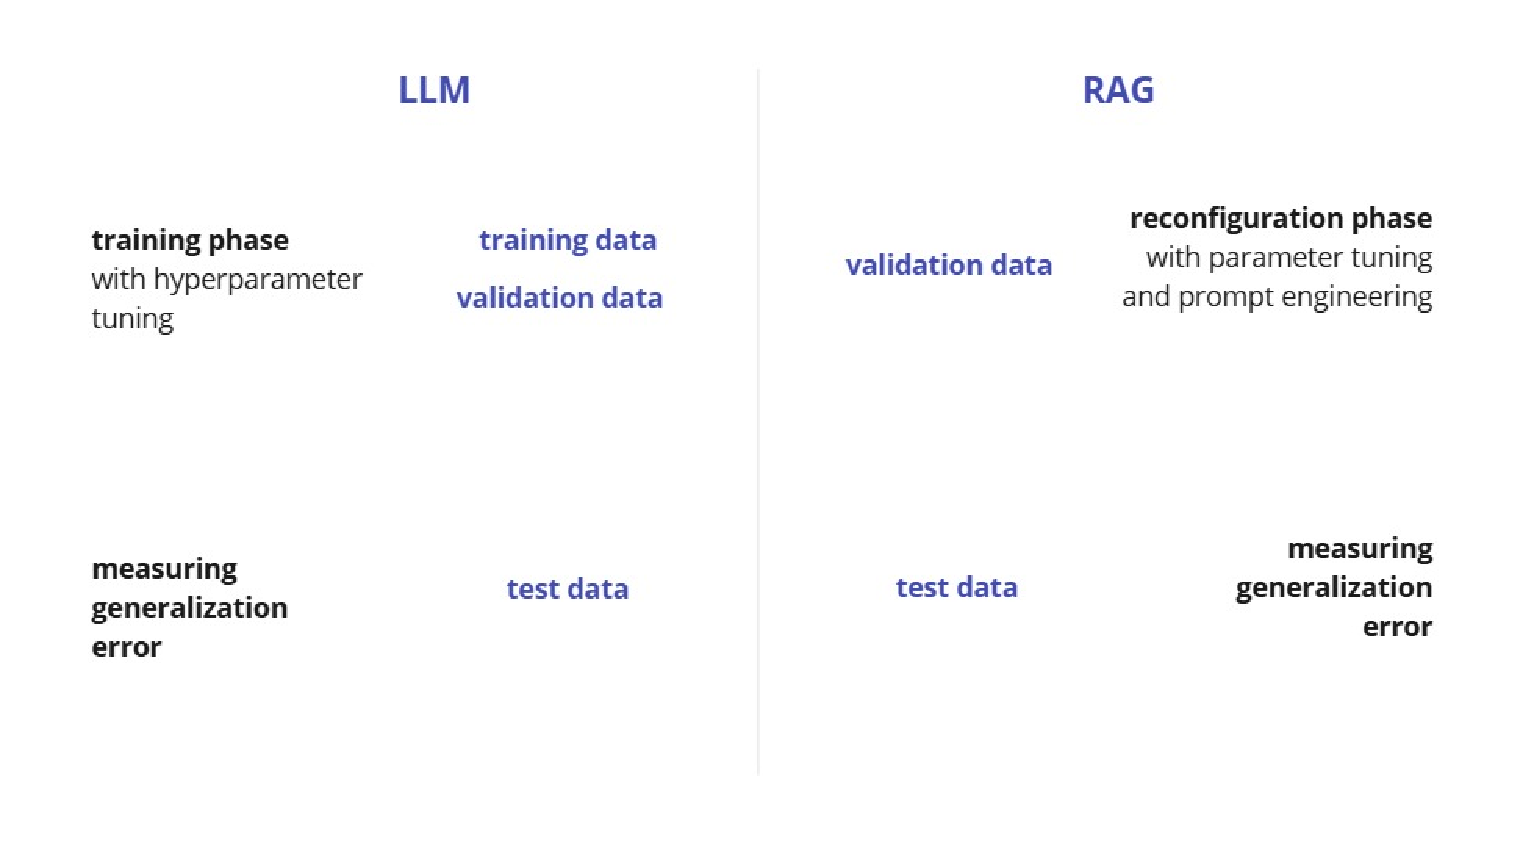
\includegraphics[width=\textwidth]{images/RAGvsLLM-tuning.pdf}
    \caption{Comparison of reconfiguration between RAGs and LLMs - both relying on tuning parameters and test data.}
    \label{fig:tuning}
\end{figure}

\paragraph{External Validity}

With our framework we handle one part of external validity concerns for RAG experimentation. We split the data into validation and test dataset so that all reconfiguration phases happen on the validation dataset, no matter if they include custom trained components or not. Only at the last stage of this development, the generalization error is estimated and the test dataset is used. Users can then compare per MLflow experiment run metrics calculated on validation data versus metrics calculated on test data. The visualisation should enlight which system configurations perform only on validation data well. 

\section{User Interface}

\begin{figure}[!ht]
    \centering
    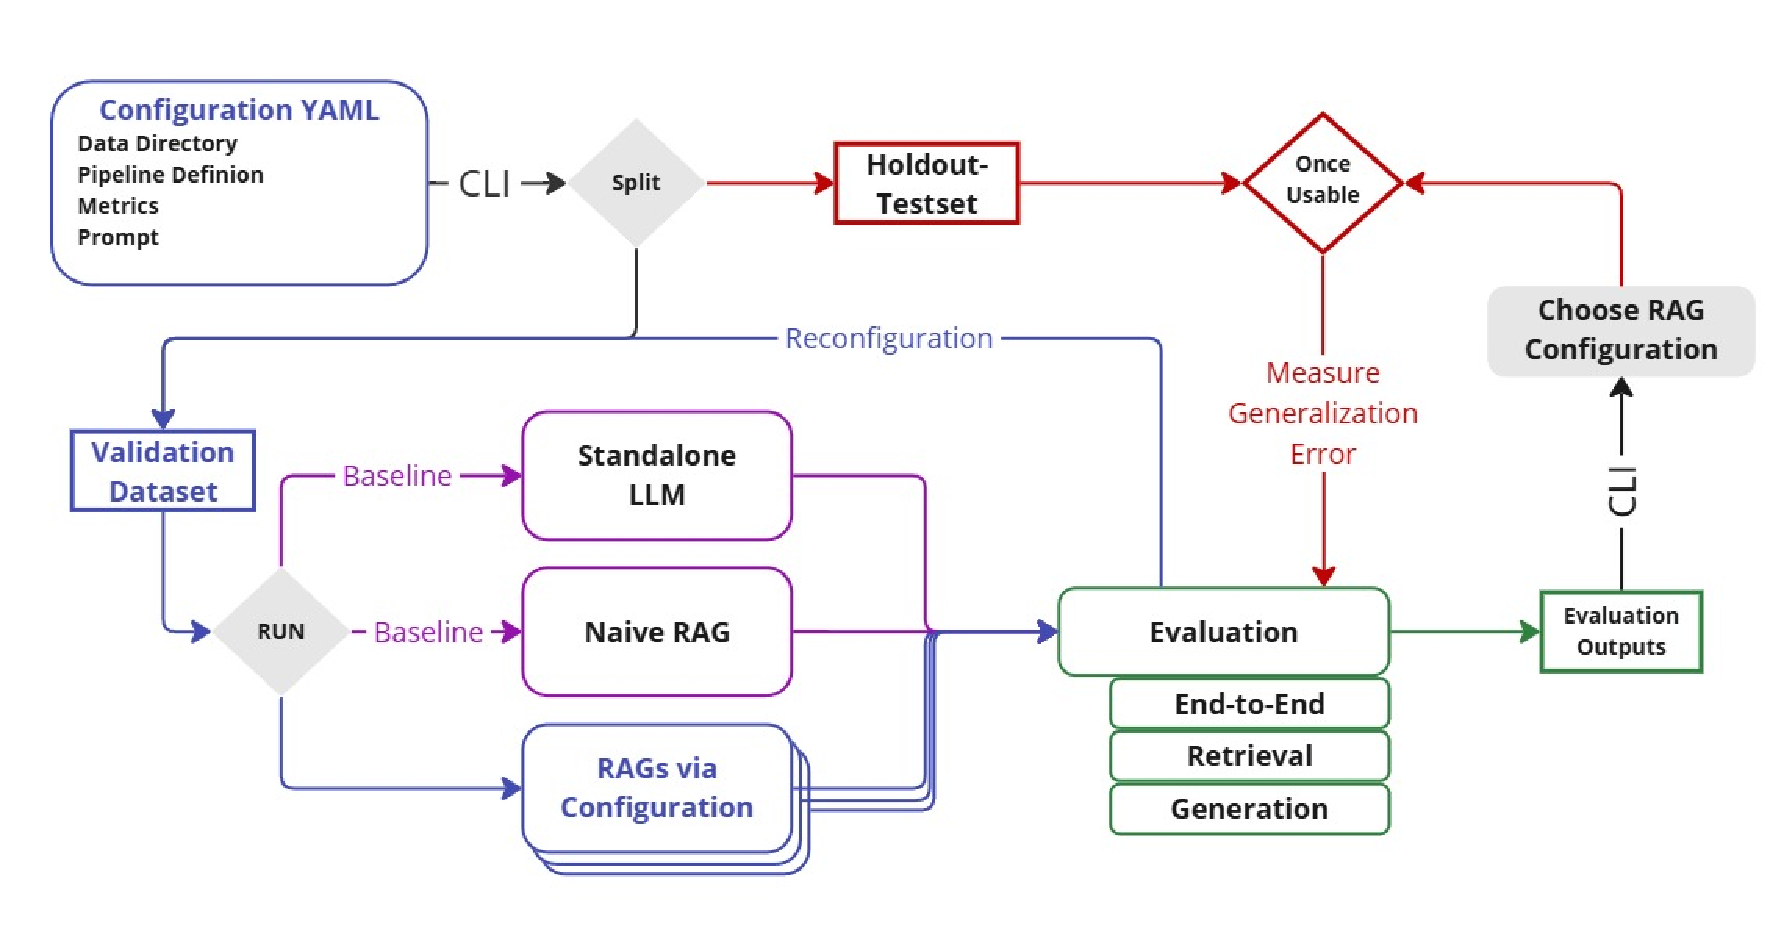
\includegraphics[width=\textwidth]{images/Sketch.pdf}
    \caption{...}
    \label{fig:EvaluationDesign}
\end{figure}

We use the presented Haystack functionalities to build a CLI-based framework around it. Our complete appraoch can be seen in figure \ref{fig:EvaluationDesign}. Given a data directory, pipeline and metrics definition, we first split the data into a validation and holdout-test dataset based on a split parameter \textit{test\_size}. Next we use the resulting validation dataset to run the first evaluations on the data. For that it loads the pipeline and data from its paths and starts with evaluating against a standalone LLM to have a baseline if RAG at all is a significant improvement in contrast to having just an LLM. Next, it ingests data into a vector database and builds an naive RAG with (Retrieve-Read) architecture as another baseline in contast to the in the YAML file defined advanced RAG architecture. The same procedure starts with the RAG configuration from the file. Each run gets evaluated in respect to End-to-End evaluation and component-wise. Evaluations are visualized in \textcolor{red}{EVAL INFOS EINFÜGEN Framework oder PRozess für Indepth Failure Analysis hier erklären}. After failure analysis, the RAG can be reconfigured again to test new parameters. 

The framework provides a command-line interface built with Typer that enables efficient RAG evaluation workflows. Two main commands are available: \textit{run-evaluations} executes experiments against baseline models (standalone LLM and naive BM25 RAG) and custom configurations defined in YAML files, with results logged to MLflow; and \textit{test-generalization-error} evaluates optimized configurations against the held-out test set. All commands integrate with Langfuse for tracing and MLflow for experiment tracking, ensuring reproducible and transparent RAG development.

\section{Limitations}

This Framework focusses primarly on classification tasks. However, the framework is expandable via custom metrics so that users could in theory define their own metrics classes for generalization tasks. 

We implemented the framework as modular as possible so that every possible architecture with all customized components can be evaluated. We can not guarantee that every architecture is possible and supporting agentic workflows might need further work.



% Some Explanatory Notes:
% Do I have to make a minimal manual here? I don't think so. I guess I have to write down What I have decided WHY

% Was unterscheidet mein Framework von existierenden?